\chapter{Approaches} \label{chap:approaches}

This chapter will describe the main dataset used for this research, why it was chosen,
the main EMG signals of interest from the dataset, methods of feature selection and
visualisation and the machine learning approaches used to transcribe the EMG data
into a text transcription.

\section{Data Preprocessing}

\subsection{Audio Speech Features}

For the purposes of the fine tuning experiments, the ground truth audio files
are preprocessed into mel spectrograms rather than MFCCs as in the original two papers
(\cite{gaddy2020digital}, \cite{gaddy2021improved}). The reason for this is because 
mel spectrograms contain more raw data than MFCCs which makes them more appropriate for
speech recognition and also the vocoder used for this paper uses mel spectrograms as the input,
as do most SOTA vocoders.

\section{Data Augmentation via EMG Synthesis}

One approach for improving the performance of any machine learning model
is to synthesize more data. This is particularly useful if the original
dataset is small and there are methods to synthesize more data.

\subsection{Related Work}

Previous approaches have used various deep learning techniques to synthesize
more EMG data to train EMG deep learning models. One approach
(\cite{gpt_2_emg_synth}) uses a GPT-2 (\cite{gpt_2_original}) like model
to synthesis EMG signals for simple action recognition such as grasp and
release (actions common to robotic prosthetics and manipulators). The inclusion
of synthesized EMG data during the training process improved the overall
gesture recognition accuracy from 68.29\% to 89.5\%.

Another related paper from the same author experiments with LSTM and GPT-2
models for synthesizing more speech for a speaker recogntion task. The
best model found by the authors for this task was a
3-layer, 128 hidden dimension LSTM network (\cite{speech_synth_lstm}).

\subsection{Research Design}

My formal hypothesis for this section is that it is possible to train
an EMG augmentation model for voiced EMG data which can improve the
performance of a regular transduction model by training on the
ground truth voiced EMG data and the synthesized voiced EMG data.

My research design involved experimenting with different hyperparameters
for my proposed network to see which values produced the lowest
loss value on the evaluation dataset. This metric was chosen as it
was the most objective measure of how the model was able to generalise
it's ability to produce novel EMG signals given a mel spectrogram input.

The loss function chosen for this task is mean squared error. This was
chosen for two reasons: firstly the original transduction model
from the Digital Voicing (\cite{gaddy2020digital}) paper uses this
loss function to transduce mel-frequency cepstrum co-efficients (MFCCs).
MFCCs are another common method of representing speech features.

Another
reason mean squared error was used was that recent research into
silent speech transduction uses an auxilliary loss function where the
transducer is given an additional task to predict the features of
the vocalised EMG input signal representation while it is presented
with a silent EMG input signal. The loss functions which the authors
chose was mean absolute error, however, they likely chose absolute
error instead of squared error because it has less of a drastic
effect on their overall loss calculation. For this task, we only
care about predicting the vocalised EMG signals given speech features
so mean squared error should provide a stronger signal to the overall
network.

\subsection{Summary}

In summary, my hypothesis was disproved.
My initial hypothesis was that it was possible to simply reverse the
transduction network, which was introduced in the Digital Voicing paper
for transcribing from EMG features into speech features, but instead
reverse the features.
From my findings I found that this wasn't true because the low level 
features of the EMG data are difficult for the LSTM network to correctly reproduce.

In hindsight my approach could have been improved by being more selective in
the early stages. I could have determined which electrode contributed the most
in the transduction task, and then tried to just synthesise the signals for that 
particular channel and then tried to synthesise an increasing number of electrode channels.

\iffalse
\section{Training an ASR System on Raw Voiced EMG Signals}
\fi

\section{Fine Tuning Speech Recognition on Model Predictions}

This section details an improved approach for training a silent speech
recognition system by pre-training a DeepSpeech2 model directly on the
predictions of a chosen portion of the dataset.

This is better than performing
speech recognition on the final waveform generated in the Digital Voicing
(\cite{gaddy2020digital}) paper.

Although the method used in that paper isn'\t
used directly for speech recognition, the end-to-end evaluation procedure
can be used for speech recognition by transducing from from the silent EMG
data into speech features, then using a vocoder to go from speech features
into an audio waveform and then using a pretrained ASR model to predict speech
from the waveform.

The proposed method skips over the vocoder entirely which improves the
end-to-end performance as there is now one less step involved.

\subsection{Related Work}

The intuition behind fine tuning a speech recognition model on the
predicted mel spectrograms from the transduction model comes
from the literature for speech recognition. Typical speech recognition models
suffer from a loss of accuracy when they are only trained on clean audio data
and then evaluated on a noisy dataset (\cite{DS2_original}). For example,
in the DeepSpeech2 paper the authors trained their speech recongition
model on different fractions of a dataset.

Their results showed that the
performance of a model trained on a clean dataset, when evaluated on a dataset
of clean audio compared to noisy audio, showed a larger gap when trained on less
data. When the authors trained their model on 1\% of the entire dataset (120 hours),
the WER for the clean dataset was 29.23\% whereas for the noisy dataset it was 50.97\%.
However when they trained on the full dataset (12,000 hours), the clean audio
WER was 8.46\% compared to 13.59\% for the noisy dataset.

The results from their paper show a strong relationship between datasize and
affect on evaluation performance on a noisy dataset. For this reason, this paper
researches the affect of providing predicted speech from the SOTA silent speech
transduction model to a speech recogntion model to improve it's performance for
speech recognition and speech synthesis (\cite{DS2_original}).

\iffalse
\subsection{Relevance to EMG Silent Speech Classification}

This issue is also reflected in the transduction task. The state-of-the-art
transduction model within the second David Gaddy (\cite{gaddy2021improved}) paper
will always produce audio outputs with artefacts because of the final vocoder layer
and because the mel spectrograms will always at best be an approximation.

This becomes problematic if you want to use the transduction model as a basis for a
speech recognition system as most pre-trained speech recognition systems
are trained on clean audio datasets which means that naively applying a speech
recognition system on top of the transduction model will result in reduced performance.
\fi

\subsection{Relation to EMG Silent Speech Classification}

\begin{figure}
  \centering
  \begin{subfigure}{.5\textwidth}
    \centering
    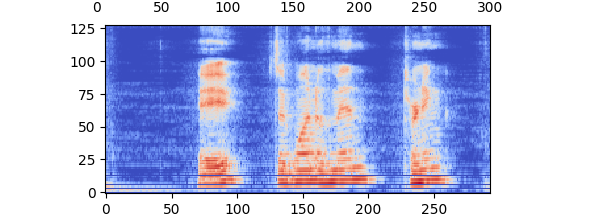
\includegraphics[width=1.\linewidth]{graphics/mel_vs_pred/ideal/458_g.png}
    \caption{Ground Truth Mel Spectrogram}
    \label{fig:sub1}
  \end{subfigure}%
  \begin{subfigure}{.5\textwidth}
    \centering
    \includegraphics[width=1\linewidth]{graphics/mel_vs_pred/ideal/458_p.png}
    \caption{Predicted Mel Spectrogram}
    \label{fig:sub2}
  \end{subfigure}
  \caption{Comparison of Ideal Ground Truth and Predicted Mel Spectrograms}
  From both of these mel spectrograms, we can see the the low level features
  of the predicted mel spectrogram appear blurrier (the curvy red lines).
  This is because the transduction model a simple linear layer (MLP) between the final
  transformer layer and the output. This limits the ability of the model to produce
  more fine tuned results. Not pictured in the figures, is
  the text transcription for utterances which is: '"Eh?" said one of the men, turning.'.
\end{figure}

\subsection{Research Question}

\subsection{Hypothesis}

My hypothesis based on my literature review, 

\iffalse
However this also opens up a new possibility, use the error correcting properties
of speech recognition systems to improve the synthesis of speech.
\fi

\subsection{Closed Vocabulary Dataset}

The closed vocabulary dataset is the first dataset used to determine how much better
a speech recognition model can be improved by training on the predicted mel spectrograms
from an already trained transduction model.

The WER of the closed vocabulary ASR model trained only on the training dataset
of the closed vocab dataset is 37\%. This means that we would not expect the WER
of the model, when it's evaluated on transduced examples, to perform better than
the ground truth word-error rate.

% (Desc.) UoP: FYP: SEMG ASR (Finetune DS2 on Transducer Outputs #8)
{\small\begin{center}
\captionof{table}{DeepSpeech2 Closed Vocab Finetuned Results}
\begin{tabular} {  l  c  c  }
\hline
\textbf{Dataset} & \textbf{CER} & \textbf{WER} \\
\hline
Ground Truth (GT) & 87.10 & 100.50 \\
Voiced & 51.27 & 87.33 \\
Silent & 38.80 & 78.10 \\
Silent, Voiced & \textbf{35.26} & 75.33 \\
\hline
Silent, Voiced, GT & 35.72 & \textbf{70.83} \\
\hline
\end{tabular}
\end{center}}

The above results do not use phonemeic prediction and only use greedy decoding
in the decoder. DeepSpeech2 is also not the SOTA model for speech recognition
which also reduces the performance. This means that the best WER of 70.83\% could
be improved upon a lot more.

For the combined silent, voiced and GT condition, the model is pre-trained on the
ground truth model and and then fine-tuned on the predictions of the
silent and voiced utterances.

Here we can see that training on predictions from both modalities from scratch
is better than training on a single modality only. However the model is only
evaluated on silent EMG text classifications which means that for this experiment,
training on silent and voiced predicted speech improves the performance when
evaluating on only the silent EMG predictions.

This may be because both of the
individual datasets are small (only 400 utterances) so doubling the dataset to
800 utterances gives the model far more examples to learn from, even though the
voiced examples diverge from the silent examples.

\subsection{Open Vocabulary (Parallel-Only) Dataset}

The next dataset used is the parallel voiced and silent EMG data. This is used because
it's smaller than using the entire open vocabulary condition dataset in one go which
makes training the individual ASR models and the transduction model faster.

The WER of the ASR model trained only on the
training dataset of the open vocabulary parallel voiced audio is 64.47\%.

% (Desc.) UoP: FYP: SEMG ASR (Finetune DS2 on Transducer Outputs #8)
{\small\begin{center}
\captionof{table}{DeepSpeech2 Open Vocabulary Parallel Finetuned Results}
\begin{tabular} {  l  c  c  }
\hline
\textbf{Dataset} & \textbf{CER} & \textbf{WER} \\
\hline
Ground Truth (GT) & 66.70 & 110.49 \\
Voiced & 156.29 & 100.00 \\
Silent & 44.21 & 84.19 \\
Silent, Voiced & 42.11 & 85.30 \\
Voiced, GT & 43.06 & 84.65 \\
Silent, GT & 41.24 & 83.97 \\
\hline
Silent, Voiced, GT & \textbf{41.02} & \textbf{81.69} \\
\hline
\end{tabular}
\end{center}}

Due to the results of the closed vocabulary training condition and time constraints,
training on the voiced portion of the open vocabulary paralell mel spectrogram
predictions wasn't conducted.

There is one interesting difference in this training run compared to the closed
vocabulary dataset. Training on the silent EMG and voiced EMG conditions together
reduces performance. This may be because training on both together was better
on training on just the silent EMG signals for the closed vocabulary dataset
because the silent EMG dataset only contained 400 data samples so doubling
the dataset to 800 data samples, even though the vocalised samples are sub-optimal,
is better. However, here the silent EMG dataset is comprised of 2,778 data samples
which means that the difference between the silent EMG and voiced EMG predicted
mel spectrograms is reducing the performance of the ASR model more than having a
larger overall dataset is beneficial.

\subsection{Open Vocabulary Full (Parallel and Non-Parallel) Dataset}

This dataset is the full entire dataset, not including the closed vocabulary
dataset. The experiments for this dataset include the same experiments for
the previous two datasets. However, extra experiments are added for the additional
non-parallel vocal EMG mel spectrogram predictions. The paralell silent and voiced
mel spectrogram predictions are included here to show how predicted speech features
from a model trained with more data improve the predictions of the same dataset.
This has the effect of making the predicted mel spectrograms closer to the ground
truth mel spectrograms which means the model is better able to classify the text
as the dataset for the entire training regime is closer to the same underyling distribution.

The WER for the ground truth model evaluted on the audio is 45\%. This means that we wouldn'\t
expect the model to have a lower WER than this value.

{\small\begin{center}
\captionof{table}{DeepSpeech2 Open Vocabulary Full Dataset Finetuned Results}
\begin{tabular} {  l  c  c  }
\hline
\textbf{Dataset} & \textbf{CER} & \textbf{WER} \\
\hline
Ground Truth (GT) & 61.99 & 100.74 \\
Parallel Voiced & -- & - \\
Silent & - & - \\
Silent, Parallel Voiced & - & - \\
\hline
Silent, Parallel Voiced, GT & 32.48 & \textbf{68.26} \\
Silent, Parallel Voiced, Non-Parallel Voiced, GT & \textbf{31.16} & 68.51 \\
\hline
\end{tabular}
\end{center}}

Here we can see that when the transduction model is trained on the full dataset,
it produces the best final WER. However there is also another interesting finding,
fine tuning the ground truth model on the silent, parallel voiced and non-parallel
voiced harms the overall WER but the CER continues to improve. This means that
the model is better able to predict individual characters but it's ability to
predict words has been slightly reduced.

\subsection{Implementation Errors}

\begin{figure}
  \centering
  \begin{subfigure}{.5\textwidth}
    \centering
    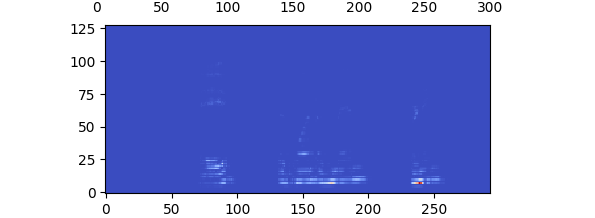
\includegraphics[width=1.\linewidth]{graphics/mel_vs_pred/real/458_g.png}
    \caption{Ground Truth Mel Spectrogram}
    \label{fig:sub1}
  \end{subfigure}%
  \begin{subfigure}{.5\textwidth}
    \centering
    \includegraphics[width=1\linewidth]{graphics/mel_vs_pred/real/458_p.png}
    \caption{Predicted Mel Spectrogram}
    \label{fig:sub2}
  \end{subfigure}
  \caption{Comparison of Real Ground Truth and Predicted Mel Spectrograms}
  From both of these mel spectrograms, we can see the the low level features
  of the predicted mel spectrogram appear blurrier (the curvy red lines).
  This is because the transduction model a simple linear layer (MLP) between the final
  transformer layer and the output. This limits the ability of the model to produce
  more fine tuned results. Not pictured in the figures, is
  the text transcription for utterances which is: '"Eh?" said one of the men, turning.'.
\end{figure}

\subsection{Summary}

In summary, this approach proves to be very successful for producing
an efficient EMG silent speech recognition system which can match the
performance of an old transducer model, re-purposed for ASR, while
the speech recognition portion of the new proposed system is only trained
on around 33 hours of data versus 3,817 (\cite{deepspeech0.7.0-training-ref}) of data.

\iffalse

\section{Dataset}

\subsection{Dataset Selection and Justification}

The dataset which is used throughout this research project is the open-source
surface electromyography silent speech (sEMG silent speech) dataset released
by David Gaddy along with his paper, Digital Voicing of Silent Speech
(\cite{gaddy2020digital}).
The paper describes a novel method of transcribing aligned silent speech data
directly into speech features along with the largest open-source sEMG silent
speech dataset.

This dataset was chosen for this research as it is the largest, high quality open
source sEMG silent speech dataset.

\subsection{Feature Selection}

For this research there were two primary ways of selecting features. The first method
was to use the same feature processing methods described in the original
(\cite{gaddy2020digital}) paper. The second method was to use a convolutional
neural network (CNN) architecture to automatically learn features from the
dataset, in an end-to-end manner.

\section{Models}

\subsection{DeepSpeech2 Model}

The DeepSpeech2 model was the initial automatic speech recognition (ASR) machine
learning model which was considered for experimentation as it is relatively simple to
implement and is known to have good performance, even on smaller datasets, achieving
a 3.10 WER on the WSJ eval'92 dataset
(\cite{DS2_original}).

\section{Baseline Audio ASR Testing}

To get a realistic baseline for the possible performance of the silent
speech models, standard audio based ASR models were trained on different
slices of the Digital Voicing datasets audio and text transcriptions only.
The intuition for this was that an ASR model trained on the audio and text
transcriptions should in theory perform better than on the purely vocalised
EMG data or final silent EMG data and their respective text transcriptions.
The results of the baseline ASR models is provided below.

\subsection{Datasets}

Three main datasets were chosen for the baseline ASR tests. The first dataset
was the LJSpeech dataset
(\cite{ljspeech17})
which is an open-source dataset primarily used in
speech synthesis and also speech recognition. The remaining two datasets
are comprised of the audio and text transcriptions of vocalised
utterances from the Digital Voicing dataset release (\cite{gaddy2020digital}).
The first dataset from this data comes from utterances from the closed
vocabulary set of recordings during the vocalised condition from the dataset.
The second dataset from this data comes from
all of the audio and text transcriptions during the vocalised condition across
the entire dataset. The three datasets are referred to as
\textit{ASR-LJSpeech}, \textit{ASR-SilentSpeechVocal-Closed} and
\textit{ASR-SilentSpeechVocal-Full},
respectively.

The \textit{ASR-LJSpeech dataset} was chosen as it is a standard open-source dataset
used for speech related machine learning tasks. It also has similar, but greater
quantity of important properties than the \textit{ASR-SilentSpeechVocal-Full} dataset.
These include the vocabulary size,
average length of recordings and duration of the entire dataset. This intuitively
means that the DeepSpeech2 ASR model trained on the \textit{ASR-LJSpeech dataset} should
have a lower WER rate, so better performance, than trained on
the \textit{ASR-SilentSpeechVocal-Full dataset}.
Whereas the \textit{ASR-SilentSpeechVocal-Closed} dataset was chosen because it has
a far lower duration and vocabulary size than the \textit{ASR-SilentSpeechVocal-Full}
dataset which makes it a lot faster to experiment with as the training time is
lower.

\subsection{Implementation}

The final DeepSpeech2 audio ASR model and training code is adapted from
online simplified examples of the original DeepSpeech2 implementation by Baidu.
Modern improvements to the model and pre-processing of the data are implemented.
These include transforming the audio waveforms into mel spectrograms and
occasionally masking parts of the spectrogram along frequency and time.

This
helps regularise the model by periodically zeroing out parts of the input.
This is similar to another regularisation technique often used in training
neural networks, known as Dropout. The goal is to reduce overfitting by preventing
complex co-adaptations on training data
(\cite{pmlr-v28-wan13}).

Another method which is used to greatly increase training speed and increase
batch size is Automatic Mixed Precision. Deep neural network training has
normally relied on IEEE single-precision format (fp32), however mixed
precision allows training with half precision (fp16, or bfloat16) while
maintaining the accuracy of single precision.

\subsection{Results}

The following results table shows the word-error rate for each dataset
which the DeepSpeech2 model was trained on. Each dataset used a slightly
different vocabulary. The vocabulary for each dataset
is the list of valid characters
of the text transcriptions which the model considers, any other characters
are encoded as \textless UNK\textgreater. A different vocabulary was chosen for the
ASR-SilentSpeechVocal-Closed dataset because it contains far more numbers
than the other datasets and including numbers in it's vocabulary means
that the transcriptions would be useful, rather than filled with the
unknown placeholder value.

% ALL OF THESE EXPERIMENTS NEED TO BE RE-RUN AT SOME POINT!

{\small\begin{center}
\captionof{table}{DeepSpeech2 Audio ASR Baseline Results}
\begin{tabular} { | l | c | c | }
\hline
Dataset & Encoding Vocabulary & WER \\
\hline
ASR-LJSpeech                 & " abcdefghijklmnopqrstuvwxyz-" & 0.55 \\
ASR-SilentSpeechVocal-Closed & " abcdefghijklmnopqrstuvwxyz0123456789-" & 0.33 \\
ASR-SilentSpeechVocal-Full   & " abcdefghijklmnopqrstuvwxyz-" & 0.45 \\
\hline
\end{tabular}
\end{center}}

\section{Vocalised EMG ASR Testing}

After training the DeepSpeech2 baseline audio ASR models, experiments
began on the vocalised EMG condition. This includes all of the utterances
in the Digital Voicing dataset where the speaker strongly articulated
what they were trying to say, or in other words, vocalised speech.
This means that the EMG signal is much stronger compared to the silent
speech condition. In theory, a model trained and evaluated on the vocalised
speech condition should show stronger performance than the silent speech
condition, due to the richer underlying signal. This means that the a dataset
comprised of purely vocalised utterances should provide a strong maximum
performance which the purely silent utterances are unlikely to be better
than.

\subsection{Implementation}

The first attempt at porting the DeepSpeech2 model from the audio ASR
condition to the vocalised EMG ASR condition involved removing the initial
CNN layers from the DeepSpeech2 model, as it was easier to just provide
the hand-crafted features from the Digital Voicing paper at first
(\cite{gaddy2020digital}). This is because it is harder to diagnose an
end-to-end deep learning model as it's not easy to visualise what the
model is doing. Then a dataset of just one sample of vocalised EMG
data from the closed vocabulary condition was setup as a training
and testing dataset. This was done to see whether or not the model
could overfit to the data. This is a standard practice done, especially
when experimenting with novel neural network architectures or domains,
because if a model cannot overfit to a single example in a dataset,
it has no chance of generalising across multiple examples and producing
useful behaviour. This is referred to as the sanity test from here on.

\fi